\documentclass{article}
\usepackage[margin=1in]{geometry}
\usepackage{graphicx}

\title{Frankenbear final documentation}
\author{Colby Goettel\and Amanda Beatty}

\begin{document}
\maketitle

\section{Introduction}
The main problem being addressed is that neither Amanda nor Colby knew too much about mechatronics and this project was a great learning platform for a variety of ideas and applications. The main things that Colby and Amanda wanted to learn about were writing embedded applications, controlling motors, using sensors to control actuators, and power consumption.

\section{Designed system}
Since the bear needs to be soft and cuddly, Frankenbear being a misnomer, is the it needed to feel right. HCI was a big concern. To solve the soft and cuddly part, light and semi-flexible components were used in the bear's big, hugging hands. A plastic, internal skeleton gave support to the body while still allowing the bear to be cuddly and approachable.

The next issue is that the bear can't be used for any creepy purposes. For this reason, there was no voice output, just lullabies, neither was a camera installed. Additionally, the light and temperature sensors were installed in an aesthetically pleasing way.

To protect the soldered wire connections, the Arduino board and the servo shield were encased in a 3D printed case with openings for power attachment, servo attachment, connections to a Raspberry Pi, and an opening for the soldered wires to exit. The case was designed by a user on thingiverse.com and printed at the ME~Checkout room in CB~154. It was a snug fit, but was effective in protecting the wiring and components.

The Arduino wiring was sufficient to complete all the tasks, until the light sensor soldering failed. After re-soldering the sensor to the micro-controller, it no longer worked. The system was difficult to repair in this regard. Proof that the sensor originally worked can be seen here:

\hfil\texttt{https://instagram.com/p/1Bz29HvzxH/?taken-by=goettels}\hfil

The servo shield was powered by AA~batteries in series. Although it required 6~V (4~batteries) it didn't work until 7.5~V were used, but the servos stopped running smoothly when 9~V were attached. The voltage supply was very trial-and-error.

The only thing that did not meet expectations is that not enough time was given to testing so power consumption was never tested. However, before the final presentation, the bear was on and used for about two hours without any sign of oncoming power failure.

\section{System analysis}
\subsection{Hardware}
The bear was controlled by an Arduino Uno R3 with a PWM shield attached. This allowed the bear to drive the four servos. The Arduino and the shield were attached and stored in a 3D printed case.

The skeleton of the bear was designed to be the least intrusive possible, while still providing stability and support for mechanical components. The skeleton consisted of a plastic rod (Ultra High Molecular Weight Polyethylene) attached to a round base plate. The base plate helped the bear to not fall over. The rod functioned as the bear's spine and supported the weight of the arm servos which were attached at the top of the rod and acted as shoulder joints. Plastic arms were attached to the servo motors which allowed the entire arm to move when the servo was actuated. After trimming down the size of the skeleton multiple times, it met our goals of being supportive without taking away the softness of the bear.

The skeleton did not require any calculations for material strength because the loads seen were so insignificant.

The ear servos were designed with a paddle that fit into the ear of the bear. The servos were light enough that they could be sewn inside the head without weighing it down. The light sensor was also attached to the crown of the head. A small hole was cut in the seam and the sensor was hot glued in place, flush with the surface. The light sensor was extremely small and exceeded our expectations in terms of visibility.

The proximity sensor had both UV and IR detection, which allowed it to be sewn to the inside of the bear's chest, unseen yet working. The proximity sensor was accurate and output repeatable data, but it would sense proximity in all directions, not just straight ahead. This presented a problem because if bear's head was pushed down, the sensor would register its closeness and the bear would start to play a song.

The PWM shield has a prototyping area where the wiring was done. Part of this wiring was the installation of a speaker that plays lullabies when the head is tickled (detected with the light sensor).

\subsection{Software}
The full code can be found on GitHub:

\hfil\texttt{https://github.com/cgoettel/frankenbear}\hfil

The C code initialized the sensors and actuators and put the arms and ears in their default position. Once the power is on, the servos are too difficult for a child to move so the arms and ears don't need to be reset at the end of every loop. Once initialized, the code looped waiting for sensors to be actuated. Functions were made for each actuation to keep the code clean.

Of note in the C code is that all printed output is controlled with a DEBUG variable, that the songs are played based off song length (not a set length), and that there are flags controlling output. These flags make it so that the bear will not continuously wiggle its ears or play songs just because the user is too close, but it will wait for the user to be farther away before it can be actuated again.

The Python code was structured in a try-catch statement that would run every needed operation unless the user aborted the program with CTRL+c.

\subsection{Development system}
The system was developed in the Arduino IDE (system independent) and in nano on the Raspberry Pi (Raspbian Linux). The embedded aspects were written in C (Arduino compiler), while the code running on the Raspberry Pi was written in Python (interpreted). Arduino libraries were used as much as possible, especially for servo control.

\subsection{Security}
Aside from what's already been stated, the only remaining security issue is that the components are all bundled together in an easy-to-steal system. Adding a \$40 GPS module isn't really worth it because of the price, but it's a thought.

\subsection{HCI}
The utility of the bear is good with the only drawback being it is not as soft or cuddly as the user might want. This would be fixed with 9~V batteries which were deemed too expensive for basic testing. The learnability and memorability of the bear is outstanding which is important since the user base will be young children. The feedback and mapping of the bear are also excellent. Everything the user does gives some sort of feedback, either mechanically or audibly, and the sensors are in intuitive locations (chest, head, and back).

The negative aspects of the bear are visibility and affordance. The button and sensors are either not visible or very well hidden, which was done on purpose so the bear does not look creepy, however this makes it difficult for the user to know what to do next. The sensors also don't allow people to know how to use them. Even if a child saw the light sensor, he would not know what to do with it to make the bear do something. This could be solved by having an initial tutorial which would lead the user through the possible uses. This tutorial could either be built into the bear's functions, or in supplied user documentation.

\section{Conclusion}
This project made a great, although heavyset, bear. All functionality as originally intended made it in with only slight modifications. The team learned each of the things they were interested in and the class was a resounding success.

The only clear goal not met was power consumption. Future work on this project would include changing the Arduino frequency to something drastically lower, although Arduino power consumption is already pretty low. Additionally, an on-off switch should be added so that the battery packs don't have to be physically disconnected whenever the bear is not in use. Finally, switching to 9~V batteries would be enough to cut weight. Cutting costs could be done with a custom printed circuit board that only had the required functionality built in.

\clearpage
\section*{Appendix: References}
\begin{enumerate}
    \item Ada, Lady. ``Adafruit 16-channel PWM/Servo Shield.'' Adafruit.com. https://learn.adafruit.com/adafruit-16-channel-pwm-slash-servo-shield
    \item Ada, Lady. ``Photocells.'' Adafruit.com. https://learn.adafruit.com/photocells
    \item Monk, Simon. ``Arduino Lesson 10. Making Sounds.'' Adafruit.com. https://learn.adafruit.com/adafruit-arduino-lesson-10-making-sounds/playing-a-scale
    \item ``VCNL4000.'' GitHub.com. https://github.com/adafruit/VCNL4000
    \item ``Arduino Uno.'' Arduino.cc. http://arduino.cc/en/Main/ArduinoBoardUno
\end{enumerate}

\clearpage
\section*{Appendix: Schematics and diagrams}
\begin{figure}[hbt]
    \centering
    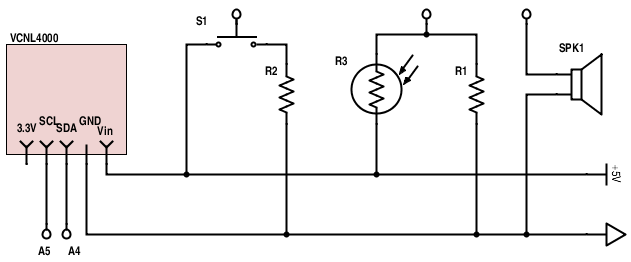
\includegraphics[width=0.8\textwidth]{schematic}
    \caption{Schematic showing the various peripherals and how they are to be connected.}
    \label{fig:schematic}
\end{figure}

\begin{figure}[hbt]
    \centering
    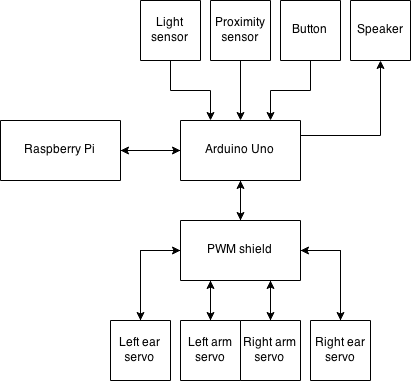
\includegraphics[width=0.5\textwidth]{block-diagram}
    \caption{Block diagram.}
    \label{fig:schematic}
\end{figure}

NOTE: Raspberry Pi connectivity is discussed in the README file in the GitHub repository.

\clearpage
\section*{Appendix: code}
C: https://github.com/cgoettel/frankenbear/blob/master/frankenbear.ino

~

\noindent Python: https://github.com/cgoettel/frankenbear/blob/master/serial.py

\end{document}
